\documentclass[11pt,center]{beamer}

\usepackage{fancybox}
\usepackage{graphics}
\usepackage{spot}
\usepackage{tikz}
\usepackage{minibox}
\usetikzlibrary{arrows}
\usepackage[absolute,overlay]{textpos}
\usetheme{metropolis}

\definecolor{light-gray}{gray}{0.86}
\title{\huge{Adaptive Machine Learning}}
\author{Βασίλειος Αταλόγλου \\ Κωνσταντίνος Σαμαράς-Τσακίρης}
\date{\today}

\begin{document}

  \begin{frame}%{\maketitle}
	  \titlepage
  \end{frame}

\section{Εισαγωγή}
  \begin{frame}{Ορισμοί}
	  Η μηχανική μάθηση αφορά την κατασκευή αλγορίθμων που μπορούν να μαθαίνουν από τα δεδομένα 				εισόδου και να κάνουν προβλέψεις σχετικά με αυτά.
	  \pause
	  \vfill
	  Διάκριση με κριτήριο τον τρόπο μάθησης σε:
		  \begin{itemize}
			  \item[--] Supervised Learning
			  \item[--] Unsupervised Learning
			  \item[--] Reinforcement Learning
		  \end{itemize}
  \end{frame}

  \begin{frame}{Παραδοσιακά νευρωνικά δίκτυα}
	  Τα συμβατικά νευρωνικά δίκτυα χρησιμοποιούν ένα τελείως απλοποιημένο μοντέλο νευρώνα που εφαρμόζει ένα σταθμισμένο άθροισμα (πχ. perceptron).\\
	  \centerline{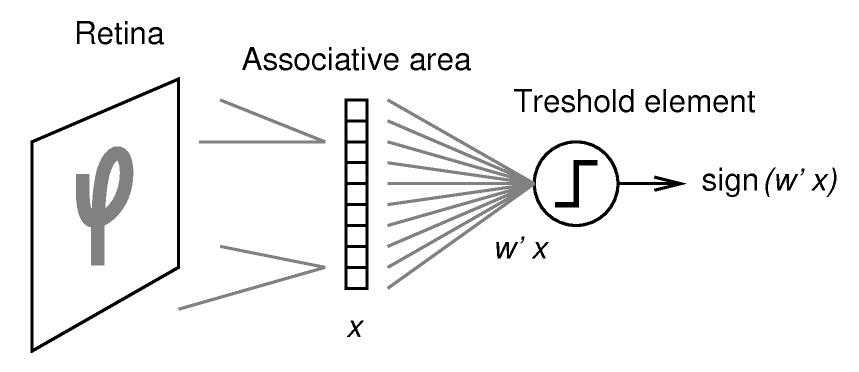
\includegraphics[width=0.4\textwidth]{../pics/perceptron.jpg}}
	  \pause
	  Ακόμα και multilayer διατάξεις (πχ. ConvNets) μπορεί να πετυχαίνουν αξιοσημείωτα αποτελέσματα αλλά μειονεκτούν σε:
	  \begin{columns}
		  \column{0.6 \textwidth}
		  \begin{itemize}
			  \item<2->[--] Χρονοβόρο training
			  \item<3->[--] Περιορισμός σε συγκεκριμένη εφαρμογή
			  \item<4->[--] Έλλειψη προσαρμοστικότητας
			  \item<5->[--] Κυρίως supervised
		  \end{itemize}
		  \column{0.4 \textwidth}
		  \\
		  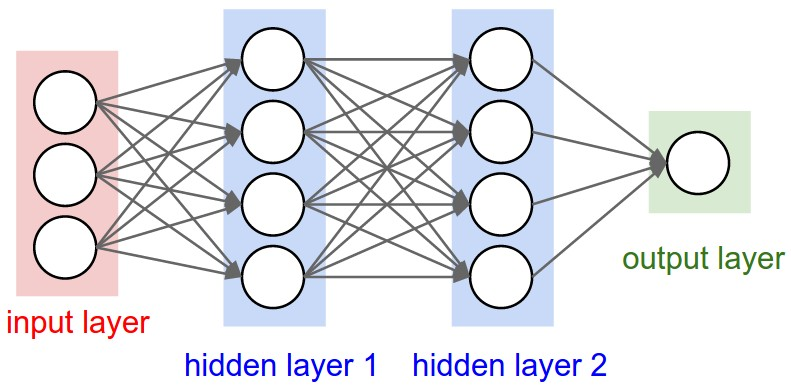
\includegraphics[width=0.95 \textwidth]{../pics/multilayer.jpeg}
	  \end{columns}
  \end{frame}

  \begin{frame}{Ανθρώπινος εγκέφαλος}
	  Αντιθέτως, ο άνθρωπος μαθαίνει \alert{συνεχώς}, έχει \alert{μνήμη} και μπορεί να κάνει 			        \alert{προβλέψεις} σχετικά με το άμεσο μέλλον.

	  \pause
	  \vfill
	  Ο ανθρώπινος εγκέφαλος είναι η αποδοτικότερη νοήμουσα μηχανή:
	  \begin{columns}
		  \column{0.6 \textwidth}
		  \vspace{-1em}
		  \begin{itemize}
			  \item<2->[--] $10^{11}$ νευρώνες
			  \item<2->[--] $10^4$ συνάψεις/νευρώνα
			  \item<2->[--] $10$ σήματα/$sec$
			  \item<2->[--] \alert{Σύνολο:} $10^{16}$ operations/$sec$!!
		  \end{itemize}
		  \vspace{+1em}
		  \begin{itemize}
			  \item<3->[--] Μόλις $25$ Watt!
		  \end{itemize}
		  \vspace{+1em}
		  \begin{itemize}
			  \item<4->[--] Ομοιομορφία σε όλη την έκταση
		  \end{itemize}

		  \column{0.45 \textwidth}
		  \\
		  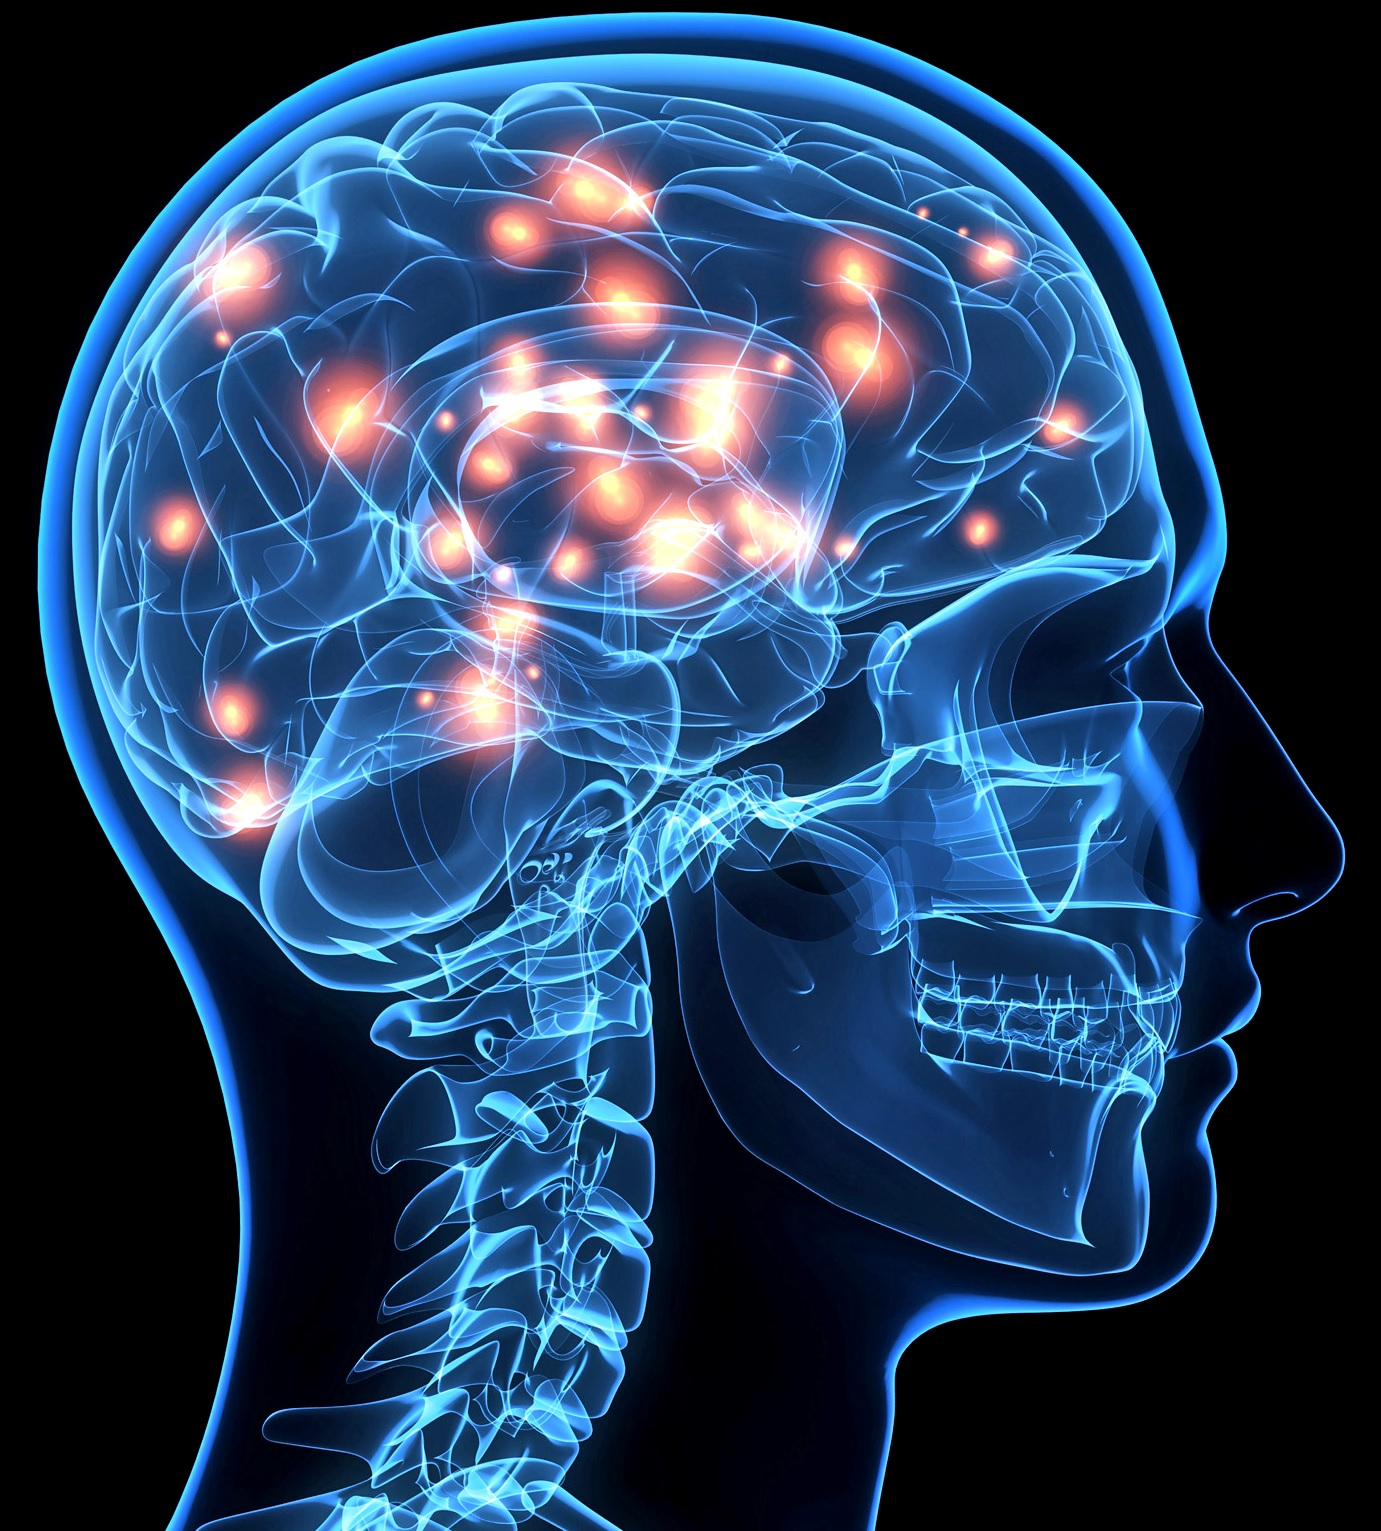
\includegraphics[width=0.95 \textwidth]{../pics/brain.jpeg}
	  \end{columns}
  \end {frame}

  \begin{frame}{Challenges}
  Συνοψίζοντας, απαίτουνται ακόμα πολλά βήματα:
  \vspace{+4em}
  \begin{itemize}
	\item[--] Online unsupervised learning (πχ. streaming data)
	\item[--] Εισαγωγή (short-term) μνήμης
	\item[--] Δυνατότητα πρόβλεψης
	\item[--] Κατάλληλο hardware
  \end{itemize}
  \end{frame}

\end{document}
